% 2009 年福建卷文科第 20 题：折叠后的三棱锥 E-ABD。
% 来源 PDF：普通高考/2009/2009福建文.pdf，SHA-256 f0a5111a6f86f4d4e8618c5c2cd0ecfd678a590b36ecbd033bb63b189700a0bc。
% 原页：第 1 页（A3 三栏）第 3 栏中部，书页码 517。
% 重绘依据：按折叠后 ED⊥平面 ABD 的构型重绘；B 在左下、D 在右下、A 在左上、E 在右上。
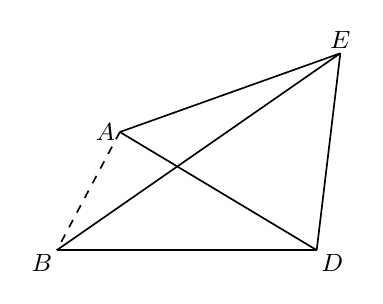
\begin{tikzpicture}[semithick, every node/.style={inner sep=1.4pt, font=\small}]
  \coordinate (B) at (0.0,0.0);
  \coordinate (D) at (3.3,0.0);
  \coordinate (A) at (0.8,1.5);
  \coordinate (E) at (3.6,2.5);
  % 可见棱
  \draw (E) -- (A);
  \draw (E) -- (B);
  \draw (E) -- (D);
  \draw (A) -- (D);
  \draw (B) -- (D);
  % 被遮挡的棱
  \draw[dashed] (A) -- (B);
  % 标注
  \node[left] at (A) {$A$};
  \node[below left] at (B) {$B$};
  \node[below right] at (D) {$D$};
  \node[above] at (E) {$E$};
\end{tikzpicture}
